% =============================================================================
\section{Lighting and Shading}\label{sec:lighting}
\subsection{Illumination model}
The light leaving a surface point is computed with the \textbf{Phong illumination model} using Blinn's half
vector (the \emph{Blinn--Phong} model). It is the sum of three reflection terms:
\begin{table}[H]
\centering\small
\caption{The three terms of the illumination model}\label{tab:phongterms}
\begin{tabularx}{\linewidth}{@{}P{1.8cm}P{4.6cm}X@{}}
\toprule
Term & Formula & Meaning \\ \midrule
Ambient & $I_a\,k_a$ & light scattered by the whole scene; it reaches every surface, also in shadow \\
Diffuse & $I_l\,k_d\,\max(\mathbf{N}\cdot\mathbf{L},0)$ & Lambert's cosine law: the brightness depends on the angle between the surface and the light, not on the viewer \\
Specular & $I_l\,k_s\,\max(\mathbf{N}\cdot\mathbf{H},0)^{n}$ & the highlight; it moves with the viewer. A large shininess $n$ gives a small sharp highlight \\
\bottomrule
\end{tabularx}
\end{table}
Here $\mathbf{N}$ is the unit surface normal, $\mathbf{L}$ the unit vector towards the light, $\mathbf{V}$ the unit
vector towards the camera and $\mathbf{H}$ the half vector,
\[
\mathbf{H} = \frac{\mathbf{L}+\mathbf{V}}{|\mathbf{L}+\mathbf{V}|},\qquad
\mathbf{R} = 2(\mathbf{N}\cdot\mathbf{L})\,\mathbf{N}-\mathbf{L}.
\]
Phong's original specular term $(\mathbf{R}\cdot\mathbf{V})^n$ uses the mirror direction $\mathbf{R}$; the half-vector
form $(\mathbf{N}\cdot\mathbf{H})^n$ gives nearly the same highlight and is cheaper to compute. For one light the model is
\[
I = I_a k_a + I_l\big(k_d\max(\mathbf{N}\!\cdot\!\mathbf{L},0) + k_s\max(\mathbf{N}\!\cdot\!\mathbf{H},0)^{n}\big).
\]
The fragment shader evaluates this sum over all active lights:
\[
C = \underbrace{\text{mix}\!\big(A_{ground},A_{sky},\tfrac{N_y+1}{2}\big)\,k_d}_{\text{ambient}}
 + \sum_{lights}\Big(k_d\max(\mathbf{N}\!\cdot\!\mathbf{L},0) + k_s\max(\mathbf{N}\!\cdot\!\mathbf{H},0)^{n}\Big)\,I\,a(d)\,c\,s
 + E .
\]
$k_d$ is the surface colour multiplied by the texture, $k_s$ the specular strength, $n$ the shininess, $I$ the
light colour times its intensity, $a(d)$ the distance attenuation, $c$ the spot-light cone factor, $s$ the shadow
factor (\Cref{sec:shadows}) and $E$ the emission of glowing surfaces. The ambient term is a \emph{hemisphere} light:
surfaces facing up receive the sky colour and surfaces facing down the ground colour. Inside the building it is
multiplied by 0.45, because the roof blocks the sky. Point and spot lights fade smoothly to zero at their
range $r$:
\[
a(d) = \frac{\big[\mathrm{clamp}(1-(d/r)^4,\,0,\,1)\big]^2}{1+d^2},\qquad
c = \mathrm{smoothstep}\big(\cos\theta_{out},\ \cos\theta_{in},\ -\mathbf{L}\cdot\mathbf{D}\big),
\]
where $\mathbf{D}$ is the spot direction and $\theta_{in}$, $\theta_{out}$ are its inner and outer cone angles.

\paragraph{Materials.} Every material carries its own $k_s$ and $n$ (\Cref{tab:materials}). Leaves and grass
use \emph{wrap} lighting, $0.6\,\mathbf{N}\!\cdot\!\mathbf{L}+0.4$, are lit from both sides, and gain a translucency term
$0.45\,k_d\,I\,s\,\max(-\mathbf{V}\cdot\mathbf{L},0)^3$ when the sun is behind them. Polished metal (bins, door
handles, wheel rims) uses a weak diffuse part $0.25\,k_d$ and a highlight in the colour of the metal, $3k_d$; it
also reflects a simple painted surrounding $E_{env}(\mathbf{R}_v)$ (sky, horizon and ground) in the mirror direction
$\mathbf{R}_v=2(\mathbf{N}\cdot\mathbf{V})\mathbf{N}-\mathbf{V}$. Car paint adds a clear-coat reflection weighted with
Schlick's approximation $F=(1-\mathbf{N}\cdot\mathbf{V})^5$:
\[
C_{metal} = C(0.25\,k_d,\ 3k_d) + E_{env}(\mathbf{R}_v)\,k_d\,(0.85+0.15F),\qquad
C_{paint} = C(k_d,\ 2.5) + E_{env}(\mathbf{R}_v)\,(0.08+0.75F).
\]
\begin{table}[H]
\centering\small
\caption{Typical material parameters}\label{tab:materials}
\begin{tabular}{@{}lcc l@{}}
\toprule
Material & $k_s$ & $n$ & Used for \\ \midrule
Fabric, plaster, bark, brick, matte & 0.03--0.05 & 6--8 & sofas, walls, trees, soil \\
Rubber & 0.08 & 8 & tyres \\
Wood, leather & 0.2--0.3 & 24 & furniture, shelves \\
Plastic, painted metal, steel & 0.35--0.6 & 48--64 & machines, keys, lamps \\
Marble & 0.6 & 96 & counter top, window sills \\
Glass & 1.0 & 160 & windows, front glass, aquarium \\
Car paint & 1.0 & 160 & cars (with clear-coat reflection) \\
Polished metal & 1.0 & 200 & bins, handles, rims (with reflection) \\
\bottomrule
\end{tabular}
\end{table}

\subsection{Light sources in the scene}
\begin{table}[H]
\centering\small
\caption{Light types used in the scene and the figures in which they can be seen}\label{tab:lighttypes}
\begin{tabularx}{\linewidth}{@{}P{1.8cm}P{3.4cm}XP{2.7cm}@{}}
\toprule
Type & Behaviour & Where in the scene & Figures \\ \midrule
Directional & same direction $\mathbf{L}$ everywhere, no attenuation & the \textbf{sun} by day and the \textbf{moon} by night & \Cref{fig:daytimes} \\
Point & radiates in all directions from a position, attenuated by $a(d)$ & lounge pendants (4), library pendants (3), ATM tube lights (2), vending machine interiors (3), ATM screen, aquarium hood, TV glow, street lamps & \Cref{fig:lampsonoff}, \Cref{fig:nightlights}, \Cref{fig:visitors} \\
Spot & a point light limited to a cone & downlights over the vending machines, the TV wall and the coffee counter, the reading lamp, porch lights, car headlights & \Cref{fig:vendbuy}, \Cref{fig:nightlights} \\
Emissive & the surface glows by itself and lights nothing else & bulbs, tubes, LEDs, screens, signs, fireflies & \Cref{fig:lampsonoff}, \Cref{fig:split_pendant} \\
Ambient & sky colour from above, ground colour from below & everywhere, changes with the time of day & \Cref{fig:lampsonoff}(b) \\
\bottomrule
\end{tabularx}
\end{table}
Every light belongs to a \emph{group}: lounge, spots, ATM room, library, outdoor or machines. Groups are switched
with the F1--F4 keys or with the light switches on the walls, and the lamp models check their group, so a bulb only
glows when its light is on. The outdoor group switches on automatically at dusk.

\begin{figure}[H]
\centering
\begin{subfigure}{0.49\linewidth}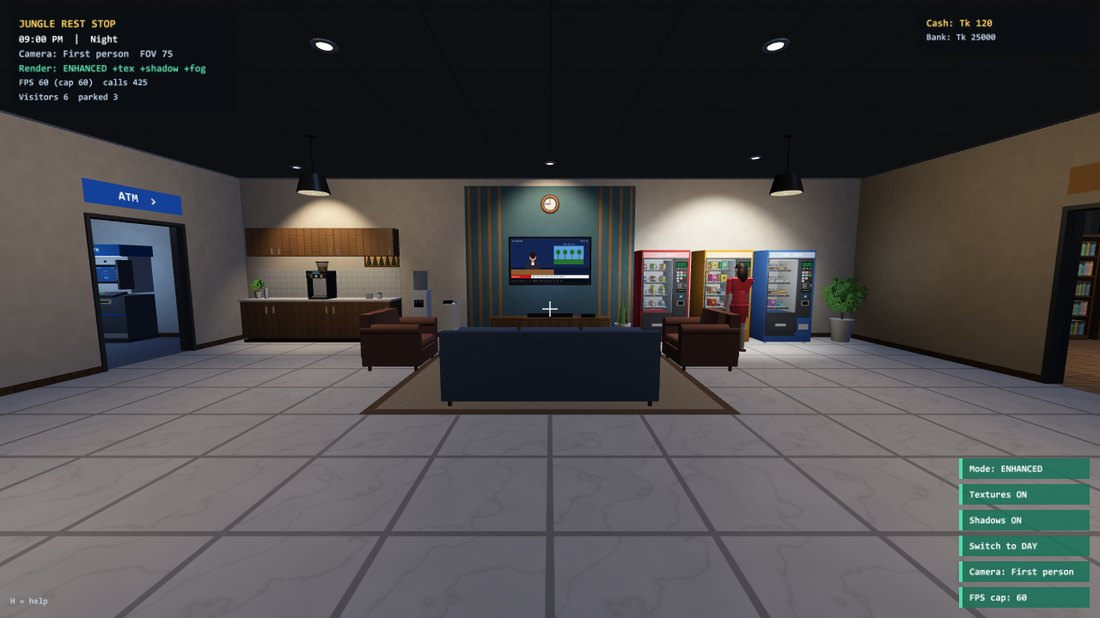
\includegraphics[width=\linewidth]{lounge_night}\caption{Night, lamps on}\end{subfigure}
\begin{subfigure}{0.49\linewidth}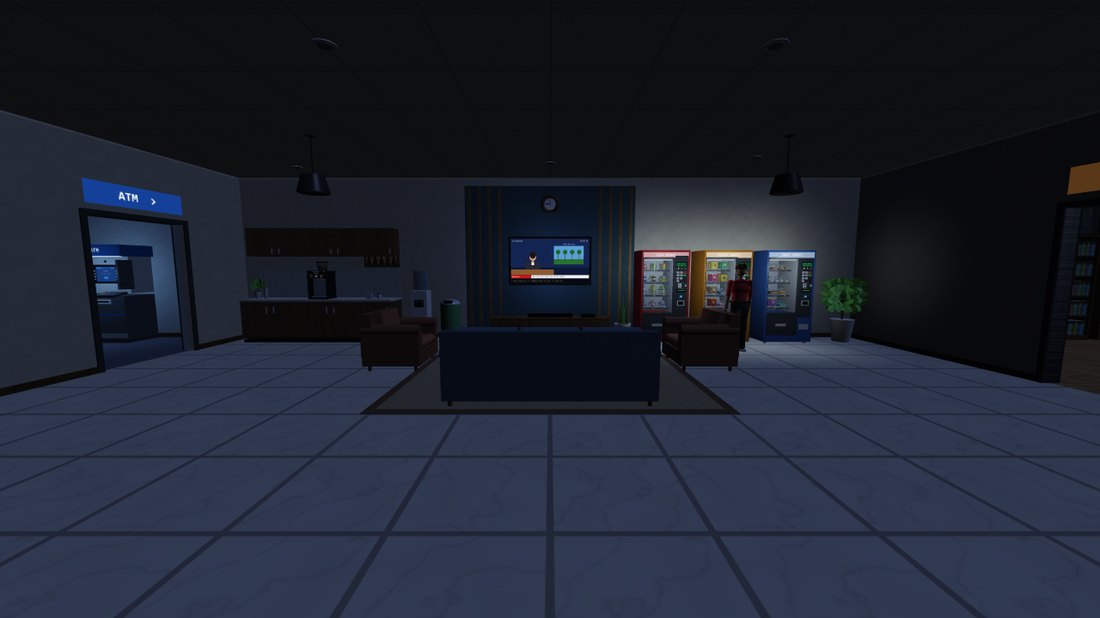
\includegraphics[width=\linewidth]{lounge_night_lamps_off}\caption{Night, lamps off (machine glow and moonlight)}\end{subfigure}
\caption{The lounge with and without its point and spot lights.}\label{fig:lampsonoff}
\end{figure}
\begin{figure}[H]
\centering
\begin{subfigure}{0.49\linewidth}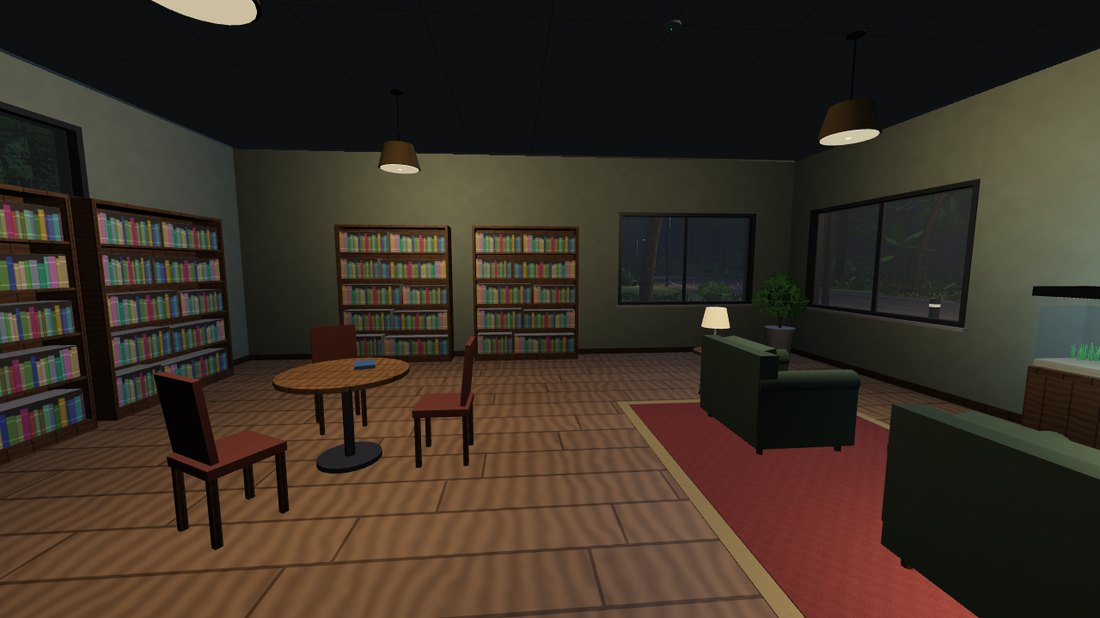
\includegraphics[width=\linewidth]{library_night}\caption{Library at night: pendants and reading lamp}\end{subfigure}
\begin{subfigure}{0.49\linewidth}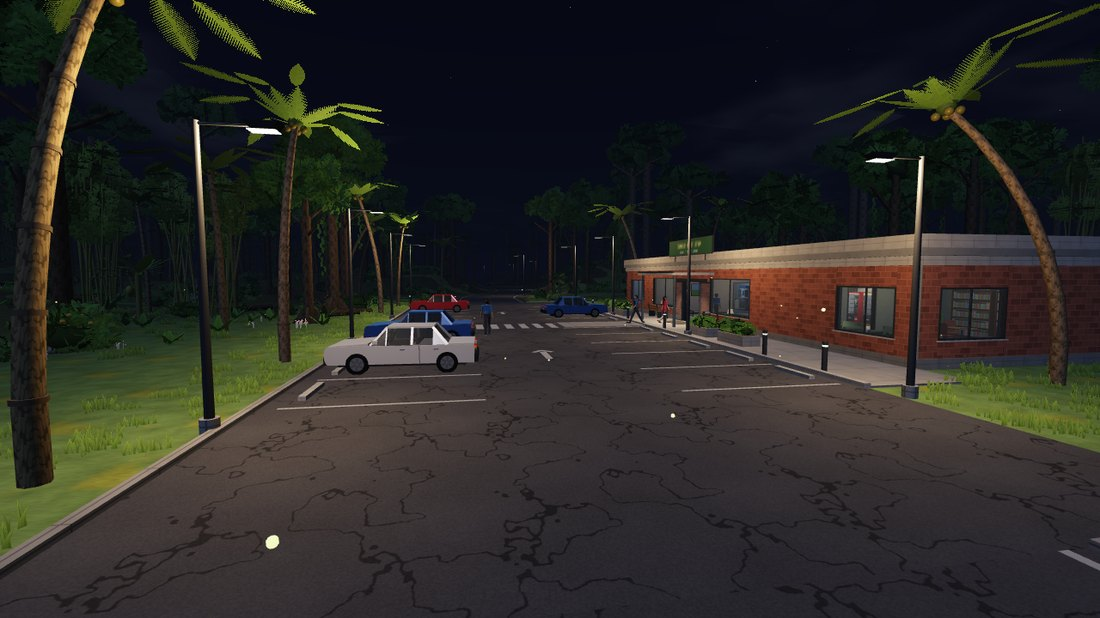
\includegraphics[width=\linewidth]{parking_night}\caption{Street lamps and car lights}\end{subfigure}
\caption{Point, spot and emissive lights at night.}\label{fig:nightlights}
\end{figure}

\subsection{Per-frame light selection}
The shader accepts up to 32 point lights and 16 spot lights. Every frame the light manager
\begin{enumerate}
  \item removes lights that are switched off or whose sphere of influence
        lies outside the view frustum,
  \item keeps the nearest ones, and
  \item sorts them by \textbf{region}: ATM room, lounge, library or outdoors.
\end{enumerate}
Each pixel determines its region from its position and loops only over the lights of that region. Light
therefore never passes through a wall into the next room, and each pixel evaluates fewer lights.

% -----------------------------------------------------------------------------
\subsection{Shading method}\label{sec:shading}
The scene uses \textbf{Phong shading}: the illumination model is evaluated once per pixel with an interpolated
normal (\Cref{fig:shadingpipe}).
\begin{figure}[H]
\centering
\begin{tikzpicture}[node distance=0.5cm,b/.style={box,text width=3.6cm,minimum height=1.6cm,font=\footnotesize}]
\node[b,fill=yellow!15] (vs) {\textbf{Vertex shader}\\$\mathbf{p}_w = M\mathbf{p}$\\$\mathbf{n}_w = N\mathbf{n}$\\$\mathbf{p}_{clip}=P\,V\,\mathbf{p}_w$};
\node[b,fill=green!12,right=of vs] (ra) {\textbf{Rasteriser}\\interpolates $\mathbf{p}_w$, $\mathbf{n}_w$, $uv$ with barycentric weights};
\node[b,fill=cyan!12,right=of ra] (fs) {\textbf{Fragment shader}\\$\mathbf{N}=\mathbf{n}/|\mathbf{n}|$\\texture, shadow\\illumination $C$, fog};
\draw[arr] (vs)--(ra); \draw[arr] (ra)--(fs);
\end{tikzpicture}
\caption{Phong shading in the OpenGL pipeline.}\label{fig:shadingpipe}
\end{figure}
\begin{enumerate}
  \item The vertex shader transforms the position into world space and the normal with the normal matrix
        $N=(M^{-1})^T$, and sends both to the rasteriser.
  \item For a pixel inside a triangle with vertices $\mathbf{p}_0,\mathbf{p}_1,\mathbf{p}_2$, the rasteriser computes the
        barycentric weights $(\alpha,\beta,\gamma)$, $\alpha+\beta+\gamma=1$, and interpolates every value
        (perspective-correct):
        \[
        \mathbf{n}(\alpha,\beta,\gamma) = \alpha\,\mathbf{n}_0 + \beta\,\mathbf{n}_1 + \gamma\,\mathbf{n}_2,\qquad
        \mathbf{p}(\alpha,\beta,\gamma) = \alpha\,\mathbf{p}_0 + \beta\,\mathbf{p}_1 + \gamma\,\mathbf{p}_2 .
        \]
  \item The interpolated normal is shorter than 1 inside the triangle, so the fragment shader normalises it,
        $\mathbf{N}=\mathbf{n}/|\mathbf{n}|$, computes $\mathbf{L}$, $\mathbf{V}=\operatorname{normalize}(\mathbf{e}-\mathbf{p})$ and
        $\mathbf{H}$, and evaluates the illumination model $C$ of the previous section for this pixel.
\end{enumerate}
Whether a surface looks smooth or faceted is decided by its vertex normals. A cube stores separate vertices for
every face with the face normal, so all pixels of a face get the same normal and the edges are sharp. A sphere or
a cylinder stores one outward normal per vertex, so the interpolated normal changes smoothly across a triangle
and the surface looks round even with 20 or 24 sides (compare the shapes in \Cref{tab:shapes}). Because the
specular term is evaluated per pixel, highlights stay sharp in the middle of large triangles, for example on
the floor tiles and on the car bonnet. The same shading is used in Basic mode, without textures, shadows and fog.
